% !TEX encoding = UTF-8
% !TEX TS-program = pdflatex
% !TEX root = ../tesi.tex

% (3) che risponde alle domande “cosa” e “come”, nel quale racconterai gli elementi essenziali del tuo stage,
% vedendolo come un mini‐progetto a se stante. In questo capitolo illustrerai: (a) il metodo di lavoro con il quale hai
% affrontato lo stage; (b) i problemi progettuali, tecnologici e applicativi che hai affrontati; (c) i risultati che hai
% raggiunto, sia sul piano qualitativo che su quello quantitativo. Il punto (a) comprende la pianificazione, le interazioni
% con il tutor aziendale, le revisioni di progresso, l’uso di diagrammi, di tecniche di analisi e tracciamento dei requisiti,
% l’uso di strumenti di verifica, ecc. Il punto (b), che tratterai nella sequenza di attività che hai svolto (analisi,
% progettazione, programmazione, verifica e validazione), metterà in luce gli aspetti principali, secondo una visione ad
% alto livello. Entrerai in dettaglio solo per aspetti che consideri particolarmente meritevoli di attenzione dal punto di
% vista delle conoscenze acquisite o necessarie. Il punto (c) tratta di copertura di requisiti, di copertura di testing, e di
% quantità di prodotti (linee di codice, numero di documenti, ecc.).


%**************************************************************
\chapter{Resoconto dello stage}
\label{cap:resoconto-stage}
%**************************************************************

\section{Descrizione del progetto}
Parte del progetto che l'azienda mi ha proposto era già stato sviluppato dal team \textit{big data} qualche anno fa.
Il \textit{dataset} da elaborare ed analizzare è infatti parte di un concorso a cui l'azienda aveva partecipato: questa competizione è stata indetta da BNP Paribas Cardif, il polo assicurativo del Gruppo BNP Paribas, e pubblicata su Keggle\footcite{https://www.kaggle.com/}, nota piattaforma in cui è possibile esporre i propri progetti, visualizzare quelli altrui e proporre sfide in ambito \textit{data science} e \textit{machine learning}.

\subsection{Il problema}
In particolare, il problema che proposto, "BNP Paribas Cardif Claims Management"\footcite{https://www.kaggle.com/c/bnp-paribas-cardif-claims-management}, consiste nella possibilità di classificare le pratiche assicurative in modo che queste possano essere risolte nel minor tempo possibile. A tal proposito, si chiede di prevedere la categoria di un sinistro sulla base delle caratteristiche disponibili nelle prime fasi del processo assicurativo; le due categorie di richieste di indennizzo, su cui basare la classificazione, corrispondono quindi a:
\begin{itemize}
	\item Quelle per le quali l'approvazione poteva essere accelerata, con conseguente maggiore rapidità nel rimborso e minori pratiche da gestire;
	\item Quelle per le quali erano richieste informazioni supplementari prima dell'approvazione e del rimborso.
\end{itemize}
\clearpage
\begin{figure}[!h] 
	\centering 
	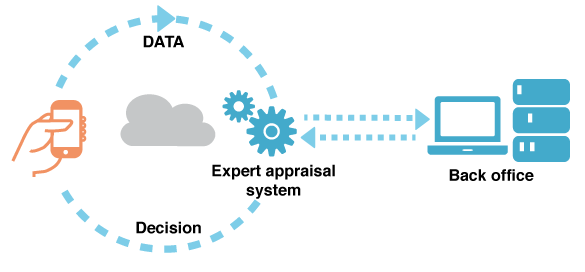
\includegraphics[width=0.7\columnwidth]{kaggle-project}
	\caption{Illustrazione del problema proposto (Fonte: \href{https://goo.gl/AW22at}{https://goo.gl/AW22at})}
\end{figure}
Nella sezione \hyperref[dataset]{Analisi del dataset di interesse} verrà trattata la struttura del \textit{dataset} più nel dettaglio.

%**************************************************************

\section{Studio di Hadoop e dei suoi tools}
L'argomento 
Prima di cominciare a lavorare sul \textit{dataset} del progetto, era necessario studiare la teoria, in quanto la prima parte dello stage considerava argomenti a me quasi totalmente sconosciuti.
Autonomamente, ma sempre supervisionato dal tutor aziendale, disponibile a risolvere ogni mio dubbio, ho studiato il materiale necessario per poter eseguire la parte pratica con la consapevolezza delle mie azioni. Oltre a ciò, nel corso della giornata lavorativa, il tutor mi sottoponeva delle esercitazioni da svolgere per consolidare i concetti appresi e risolvere tempestivamente miei eventuali dubbi prima di procedere con gli argomenti successivi.
Essendo \gls{HDFS} e molti dei tool Hadoop eseguibili principalmente tramite \gls{bash}, come prima cosa mi è stato assegnato lo studio autonomo di alcuni paragrafi, selezionati dal tutor, del libro "Learning the bash Shell"\footcite{http://shop.oreilly.com/product/9780596009656.do} per ottenere le basi che mi permettessero di utilizzare i comandi che mi sarebbero serviti in seguito per l'utilizzo dei tool Hadoop.\\
Dopo aver assorbito i concetti, già in parte di mia conoscenza, il tutor mi ha esposto la struttura del \gls{cluster} Hadoop in cui risiedevano i dati e venivano eseguiti i \textit{task}.

%**************************************************************
\section{Analisi del dataset di interesse} \label{dataset}

%**************************************************************

\section{Progettazione e sviluppo della web app}
